\documentclass[runningheads]{llncs}

% \usepackage{draftwatermark}
% \SetWatermarkColor{gray!40}
% \SetWatermarkFontSize{3cm}
% \SetWatermarkText{ Ne pas modifier !}

\bibliographystyle{splncs04}% the mandatory bibstyle

\usepackage[utf8]{inputenc} % allow utf-8 input
\usepackage[T1]{fontenc}    % use 8-bit T1 fonts
\usepackage{hyperref}       % hyperlinks
\usepackage{url}            % simple URL typesetting
\usepackage{booktabs}       % professional-quality tables
\usepackage{amsfonts}       % blackboard math symbols
\usepackage{microtype}      % microtypography
\usepackage{enumitem}
\usepackage{tikz}
\usetikzlibrary{snakes,arrows,shapes}

\usepackage{amsmath,amssymb}
\usepackage{stmaryrd}
%\usepackage{enumitem}
%\setlist{nosep}
\usepackage{mathtools}

\usepackage[]{algorithm}
\usepackage{etoolbox}\AtBeginEnvironment{algorithmic}{\footnotesize}
\def\NoNumber#1{{\def\alglinenumber##1{}\State #1}\addtocounter{ALG@line}{-1}}
\usepackage[noEnd]{algpseudocodex}
\algrenewcommand\alglinenumber[1]{\scriptsize #1}
\usepackage{caption}

\usepackage{array,multirow,makecell,diagbox}
\setcellgapes{1pt}
\makegapedcells
\newcolumntype{R}[1]{>{\raggedleft\arraybackslash }b{#1}}
\newcolumntype{L}[1]{>{\raggedright\arraybackslash }b{#1}}
\newcolumntype{C}[1]{>{\centering\arraybackslash }b{#1}}

\usepackage{graphicx}
\usepackage{wrapfig}
\usepackage{cleveref}

% unnumbered theorem-like environments used in the text
\spnewtheorem*{remark*}{Remark}{\itshape}{\rmfamily}
\spnewtheorem*{remarks*}{Remarks}{\itshape}{\rmfamily}
\spnewtheorem*{fact*}{Fact}{\itshape}{\rmfamily}
\spnewtheorem*{example*}{Example}{\itshape}{\rmfamily}
\providecommand{\qedhere}{}% amsthm command not provided by llncs


\newcommand{\cs}{\texttt{cs}}

%
%
%% A supprimer plus tard
\newcommand{\noteAnt}[2][]{\textcolor{red}{\textsc{Note de Antoine #1:} \emph{#2}}}
\newcommand{\noteSi}[2][]{{\footnotesize \textcolor{blue}{\textsc{Note de Simon #1:} \emph{#2}}}}
\newcommand{\noteMe}[2][]{{\footnotesize \textcolor{violet}{\textsc{Note de Mehdi #1:} \emph{#2}}}}
\newcommand{\MP}[1]{\marginpar{\textcolor{red}{\footnotesize #1}}}
%%



\begin{document}

\title{Exact Integer Alias Method: Robust and Error-Free Large-Scale Sampling}

\titlerunning{Exact Integer Alias Method: Robust and Error-Free Large-Scale Sampling}

\author{Oriane Crouzet\inst{1} \and
Simon Dreyer\inst{2} \and
Antoine Genitrini\inst{1} \and
Mehdi Naima\inst{1}}

\authorrunning{O. Crouzet et al.}

\institute{Sorbonne Université, CNRS, LIP6, F-75005 Paris, France\\
\email{Oriane.Crouzet@lip6.fr, Antoine.Genitrini@lip6.fr, Mehdi.Naima@lip6.fr} \and
Université de Montpellier, CNRS, LIRMM, F-34095 Montpellier, France\\
\email{Simon.Dreyer@lirmm.fr}}

\maketitle

\begin{abstract}
Walker's Alias Method, made linear by Vose, is the gold standard for sampling from a fixed discrete
distribution in constant time, but its reliance on floating-point arithmetic makes it unreliable once
weights exceed double-precision resolution, a regime already reached by applications such as combinatorial
chemistry. Existing remedies either fall back on costly arbitrary-precision arithmetic, like the Rust
\texttt{weighted\_rand} crate. We introduce the Integer-Alias Sampler, a construction and sampling scheme that
operates natively and exclusively on arbitrary-precision integer weights. We prove its correctness, give tight bounds on the resulting table size, and analyze the random-bit
consumption of the associated generator. Experiments, including a large-scale combinatorial-chemistry case
study, show our sampler achieves the best available trade-off between sampling time, memory footprint, and
randomness consumption once weights genuinely require arbitrary precision.
\keywords{Alias method \and Exact random sampling \and Arbitrary-precision arithmetic \and Discrete random variate generation.}
\end{abstract}



\section{Introduction}
\label{sec:intro}

Sampling a discrete object from a prescribed, possibly non-uniform, distribution is a recurring primitive
in computational science, underlying Monte Carlo simulation, agent-based modeling, and the stochastic
components of modern machine learning pipelines, where billions of independent draws must be produced
under strict time and memory budgets. The related question of generating or sampling from a large,
implicitly described universe of discrete structures has likewise been studied extensively, from the
classical treatises of Nijenhuis and Wilf~\cite{NW75} and Kreher and Stinson~\cite{KS99} to Ruskey's
survey~\cite{Ruskey03}, more recent developments~\cite{GP21}, and Skiena's algorithmic
toolbox~\cite{Skiena20}. In practice, the objects to be generated are rarely equally likely: they carry
integer or rational \emph{weights}, and an unbiased sampler must reproduce the corresponding distribution
exactly, however skewed it is.

The reference solution to this weighted sampling problem is Walker's \emph{Alias
Method}~\cite{Walker74,Walker77}: it reorganizes a set of $n$ unequal probabilities into $n$ buckets of
equal capacity, each holding at most two outcomes, a primary value and its designated \emph{alias}, so that
a single bucket, drawn uniformly at random, together with one biased coin flip, suffices to recover the
target distribution. Vose later showed how to build this table in linear time~\cite{Vose91}, and Smith and
Jacobson provided a thorough analysis of the resulting sampler~\cite{SJ05}. By front-loading the whole
complexity of the distribution into a one-time linear-time preprocessing step, the Alias Method achieves
$O(1)$ sampling independently of $n$, making it the gold standard whenever a fixed distribution must be
queried a very large number of times. This is the setting of this paper: the distribution never changes, and
every sampler we consider works in two phases, a preprocessing step performed once, then a sampling step
repeated as many times as needed, each with its own time and memory cost.

This efficiency, however, is traditionally obtained at the price of floating-point arithmetic, and modern
computational-science workloads increasingly expose the fragility of this choice. Both the construction of
the table and the sampling step rely on repeatedly comparing and renormalizing probabilities represented as
IEEE~754 doubles, so that rounding drift can silently corrupt the classification of outcomes during
preprocessing, and bit-creep can corrupt the coin-flip threshold during sampling. As soon as the total
weight of a distribution exceeds $2^{53}$, the granularity of double-precision floats becomes coarser than
the weight of individual items, which then acquire a \emph{structurally zero} probability of ever being
drawn. Such regimes are no longer isolated cases: in combinatorial chemistry, the space of chemically
plausible molecules grows so quickly with the number of atoms that it must be sampled rather than
enumerated, with reference libraries already ranging from about $10^{8}$ molecules for the smallest
structures to several trillion compounds for modern make-on-demand libraries~\cite{SSHL26}, well beyond
$2^{64}$ for molecules of about thirty heavy atoms. Monterrubio-Chanca and von Rudorff~\cite{MR25}, whose
open-source \texttt{nablachem} package~\cite{nablachem} we use in our own experiments, address this regime
with a pipeline whose final step is precisely a weighted random draw among combinatorial groups, over
weights of several hundred bits, well beyond the reach of a double-precision mantissa.

Several directions have been explored to make the Alias Method robust to this kind of scale. The most
direct remedy is to abandon floating-point numbers altogether and represent probabilities as
arbitrary-precision rational fractions, which restores mathematical exactness but incurs a substantial
overhead in both running time and memory, since every comparison and table entry now manipulates a pair of
big integers. An alternative, adopted by the Rust ecosystem's \texttt{weighted\_rand} crate~\cite{Rust25},
is to restrict the input to non-negative integer weights, so that the whole construction can be carried out
with exact integer arithmetic; this avoids fractions entirely, but since its construction departs from Vose's, its correctness does not
follow from Vose's proof and had, to the best of our knowledge, never been established in the literature, and, as we show in \Cref{sec:algo}, it also produces
alias tables with systematically fewer alias-free cells than Vose's construction, which slows down the
sampling step. Orthogonally, entropy-optimal samplers such as \textsc{Fldr}~\cite{SFRM19} and its
refinement \textsc{Aldr}~\cite{DS26} build on the discrete-distribution-generating trees of Knuth and
Yao~\cite{KY76} to approach the information-theoretic minimum number of random bits per sample, at the cost
of a preprocessing and sampling cost that grows with the entropy of the distribution, again without native
support for arbitrary-precision weights.

In this paper we introduce the \emph{Integer-Alias Sampler}, a construction and sampling scheme that
operates natively and exclusively on arbitrary-precision integer weights, without ever resorting to
floating-point numbers or rational fractions. We revisit Walker and Vose's construction in this exact
integer setting, formally establish the correctness of the Rust integer-weight variant~\cite{Rust25}, and
prove that our own construction, built around a natural integer cell size, yields alias tables with more
alias-free cells, and hence a faster sampling step, together with matching tight bounds on the size of the
resulting table (\Cref{sec:walker,sec:algo}). We design an efficient random generation procedure on this
table, together with a virtual-object rejection mechanism, and analyze its random-bit consumption against
the information-theoretic optimum realized by Lumbroso's algorithms~\cite{Lumbroso13} (\Cref{sec:gen}). We
implement all of the above under arbitrary-precision arithmetic, coupled with a background thread that
continuously refills a cryptographically secure random-bit stream, overlapping bit generation with sampling, supporting
distributions whose number of objects and individual weights can both grow without any fixed-width bound.
Finally, we experimentally compare our approach against the Fraction-Alias sampler, the Rust-Alias
sampler~\cite{Rust25}, and arbitrary-precision adaptations of \textsc{Fldr}~\cite{SFRM19} and
\textsc{Aldr}~\cite{DS26}, including a large-scale combinatorial-chemistry case study derived
from~\cite{MR25,SSHL26}, showing that our sampler achieves the best available trade-off between sampling
time, memory footprint, and random-bit consumption once weights genuinely require arbitrary precision
(\Cref{sec:exp}).


\section{Alias algorithm beyond floating numbers rounding errors}
\label{sec:walker}

The \emph{Alias Method}, designed by Walker in consecutive papers~\cite{Walker74,Walker77}, represents a fundamental shift
in how we sample from discrete probability distributions.
His somehow geometric approach transforms 
a set of $n$ unequal probabilities into $n$ uniform buckets of equal capacity. 
By reallocating the surplus from high-probability outcomes to fill the deficits of low-probability ones,
Walker demonstrated that any distribution can be restructured so that each bucket contains at most two outcomes: 
a primary value and its designated \emph{alias}. This structure allows for an exceptionally fast sampling process
operating in constant time, regardless of the total number of possible outcomes, as it only requires 
picking a bucket uniformly at random and performing a single biased coin flip to determine the result
(i.e. which of the two elements from the bucket to return).

While Walker’s sampling approach is extremely smart, the algorithm’s modern efficiency is largely attributed
to Vose’s 1991 refinement, which introduced a linear-time construction method for the bucket table.
This phase will be called \emph{preprocessing} in what follows. In his paper~\cite{Vose91},
Vose optimized this process to linear time in the number of elements by utilizing two worklists,
(implemented as stacks for example), to classify the outcomes as either small or large relative to the mean. 
The systematic pairing of underfilled and overfilled buckets
ensures a stable and computationally lean initialization, improving the super linear time
complexity preprocessing proposed by Walker.
Consequently, Vose’s approach transformed the Alias Method into a highly scalable tool, 
making it the definitive choice for high-performance computing and large-scale simulations.

The synergy between Walker’s conceptual framework and Vose’s preprocessing optimization makes 
the Alias Method the gold standard for scenarios requiring massive numbers of samples from a fixed distribution. 
Its ability to maintain the same execution speed whether dealing with ten or ten million objects gives 
it a distinct advantage over traditional binary search methods, which inevitably slow down as the dataset grows.

The practical implementation of the Alias Method must contend with the realities of finite-precision floating-point arithmetic, 
which introduces subtle vulnerabilities during both the construction and simulation phases. During table initialization, 
the iterative process of normalizing probabilities and reallocating surpluses can lead to precision drift, where cumulative 
rounding errors cause the total probability mass to deviate from unity or result in the misclassification of outcomes into the worklists. 
These inaccuracies persist into the simulation phase, where the sampling step relies on comparing a generated random 
variable (with a given precision) against a threshold that may have been slightly corrupted by bit-creep. Even a microscopic deviation 
(such as a probability intended to be exactly $1.0$ being stored as an infinitesimally smaller fraction) 
can erroneously trigger the alias outcome, while the discrete granularity of the underlying pseudo-random number 
generator can further distort the intended statistical distribution over the course of massive Monte Carlo trials.

To address rounding errors in both the preprocessing and simulation phases, the most effective approach
is to replace standard floating-point arithmetic with arbitrary-precision fractions.
In practice, since the floating number have finite precision, the probabilities can be represented as rational numbers, i.e. as fractions of arbitrary size. 
This technique effectively treats the input as a mathematically perfect probability distribution
(without any consideration on approximations in the inputs), eliminating the precision drift and 
bit-creep that typically plague massive Monte Carlo trials. By maintaining exact rational representations,
the software ensures that the statistical integrity of the simulation remains uncompromised, 
regardless of the number of iterations performed.
An adaptation of Vose's preprocessing is presented in~\Cref{algo:preprocessing} through the function \textsc{Table\_Fractions}. Due to the fact that no rounding error occur, the code
is simpler than Vose's original implementation.
However, relying on exact rational arithmetic introduces significant computational overhead and 
increased memory usage compared to native floating-point types, which impact
overall performance in large-scale simulations.

To improve this aspect, developers for the Rust programming language proposed 
an alternative approach~\cite{Rust25},
relying on a distribution of the objects based on some non-negative integer weights.
This restriction is directly reflected in the probability distribution of the objets, because the probability of any given object is then
a rational number. Rust's adaptation consider a sequence $S = [x_0, x_1, \dots x_{n-1}]$ of $n$ distinct objects and a sequence 
$W =[w_0, \dots, w_{n-1}]$ of non-negative integers such that object $x_i$ is of weight $w_i$. 
We denote the total weight by $w = \sum_i w_i$.

We aim at generating at random an object $x_i$
according to the global distribution $W$, i.e. the probability for generating $x_i$ is given 
by $w_i / w$, for each $i$. Obviously the later distribution is a probability distribution.
Say differently, a sequence of objects with rational probabilities can be equivalently represented with non-negative integer weights
replacing each probability $p_i$ by the integer $w_i = p_i \cdot LCM$ where $LCM$ is the least common multiple of the denominators 
of the probabilities $(p_i)_i$.

Only the preprocessing phase of the Rust implementation is distinct from the original Alias method, 
the sampling phase remains identical.
We put together both approaches in~\Cref{algo:preprocessing} for a better comparison.
Note that the Rust implementation takes advantage of polymorphism, hence the same implementation should apply either for floating point numbers, but also for integer weights distributions.
So in the following we simplify a little the pseudo-code for focusing only on necessary parts used for an integer distribution weights for objects.

The inputs are $X$ and $W$; we deduce $n$ the number of objects of $X$ and $w$ the cumulative weight of all objects. We aim at producing a table $T$ of $n$ buckets, each one with the same capacity ($1$ in Vose's case and $w$
for Rust).
Each bucket is a triplet of the form $(w', x', x)$  where, for Rust, $w'$ is the weight of the object $x'$ in the bucket and $x$ is the alias of $x'$ (implicitly, the weight of $x$ in the bucket is $w - w'$). 
For Vose, $w'$ is the probability for choosing $x'$ in the bucket , and this $1-w'$ the one for $x$, the alias.

\begin{algorithm}[htb]
\caption{Building of the Alias Tables by Vose (adaptation for fractions) and by Rust language} 
\label{algo:preprocessing}
    \begin{tabular}{l l}
        \begin{minipage}{0.52\textwidth}
            \begin{algorithmic}[1]
                \scriptsize
                \renewcommand{\algorithmicrequire}{\textbf{Input:}}
                \renewcommand{\algorithmicensure}{\textbf{Output:}}
                \Require $X$, $W$, $n$ previously defined.
                \Ensure  The table of triplets $T$.
                \Function{Table\_Fractions}{$X, n, W$}
                    \State $T = \texttt{init}(n)$ %\Comment{Initialization of a table indexed from $0$ to $n-1$}
                    \For{$x \in X$}
                        \State $W[x] = n \cdot W[x]$ %\Comment{$W[x]$ is the weight of $x$}
                    \EndFor
                    \State $L = \{x \in X \quad | \quad W[x] > 1\}$ %\Comment{$L$ is the stack of the larger objects}
                    \State $S = \{x \in X \quad | \quad W[x] \leq 1\}$ %\Comment{$S$ is the stack of the smaller objects}
                    \State $k = 0$
                    \While{$L$ is not empty}
                        \State $x = \texttt{pop}(L)$ %\Comment{pop operation extracts one object from the stack}
                        \State $x' = \texttt{pop}(S)$ 
                        \State $T[k] = (W[x'], x', x)$
                        \State $W[x] = W[x] - (1 - W[x'])$
                        \If{$W[x] \leq 1$}
                            \State $\texttt{push}(S, x)$ %\Comment{push operation adds one object to the stack}
                        \Else
                            \State $\texttt{push}(L, x)$
                        \EndIf
                        \State $k = k + 1$
                    \EndWhile
                    \While{$S$ is not empty}
                        \State $x = \texttt{pop}(S)$
                        \State $T[k] = (1, x, \emptyset)$
                        \State $k = k + 1$
                    \EndWhile
                    \State \Return $T$
                \EndFunction
            \end{algorithmic}   
        \end{minipage}
        &
        \begin{minipage}{0.5\textwidth}
            \begin{algorithmic}[1]
                \scriptsize
                \renewcommand{\algorithmicrequire}{\textbf{Input:}}
                \renewcommand{\algorithmicensure}{\textbf{Output:}}
                \Require $X$, $W$, $n$ and $w$ previously defined.
                \Ensure  The table of triplets $T$.
                \Function{Table\_Rust}{$X, n, W, w$}
                    \State $T = \texttt{init}(n)$ %\Comment{Initialization of a table indexed from $0$ to $n-1$}
                    \For{$x \in X$}
                        \State $W[x] = n \cdot W[x]$ %\Comment{$W[x]$ is the weight of $x$}
                    \EndFor
                    \State $L = \{x \in X \quad | \quad W[x] \geq w\}$ %\Comment{$L$ is the stack of the larger objects}
                    \State $S = \{x \in X \quad | \quad W[x] < w\}$ %\Comment{$S$ is the stack of the smaller objects}
                    \State $k = 0$
                    \While{$S$ is not empty}
                        \State $x = \texttt{pop}(L)$ %\Comment{pop operation extracts one object from the stack}
                        \State $x' = \texttt{pop}(S)$ 
                        \State $T[k] = (W[x'], x', x)$
                        \State $W[x] = W[x] - (w - W[x'])$
                        \If{$W[x] < w$}
                            \State $\texttt{push}(S, x)$ %\Comment{push operation adds one object to the stack}
                        \Else
                            \State $\texttt{push}(L, x)$
                        \EndIf
                        \State $k = k + 1$
                    \EndWhile
                    \While{$L$ is not empty}
                        \State $x = \texttt{pop}(L)$
                        \State $T[k] = (w, x, \emptyset)$
                        \State $k = k + 1$
                    \EndWhile
                    \State \Return $T$
                \EndFunction
            \end{algorithmic}      
        \end{minipage} 
    \end{tabular}
    \begin{itemize}
        \scriptsize
        \item $\texttt{init}(n)$: Initialization of a table indexed from $0$ to $n-1$
        \item $L$ is the stack of the larger objects; $S$ is the stack of the smaller objects
        \item $\texttt{pop}(\cdot)$: pop operation extracts one object from the stack
        \item $\texttt{push}(\cdot, \cdot)$: push operation adds one object to the stack
    \end{itemize}
 \end{algorithm}

Vose established the algorithm's correctness for exact arithmetic by proving that $S$ cannot be exhausted before $L$. 
This ensures that any objects remaining at line 18 have a weight of exactly 1 and require no alias. 
Rust's implementation differs: after scaling by $n$, an object whose weight equals the cell capacity $w$ (that is, an object of exactly average weight $w/n$) is classified as large (put in $L$). Intuitively,
this change should give more possibilities to complete smaller objects, thus the correctness
should not be affected.
But to the best of our knowledge, this approach provided by Rust has not been proved correct in the literature.
Furthermore, in the implementation the loop condition (line 8) is different \texttt{while S and L are not empty}, and also there is third loop, line 22 to empty the stack $S$.
We will prove it is non necessary in the context of integer weights distribution.

\begin{proposition}
    Rust algorithm is correct for the building of the Alias Table.
\end{proposition}
The proof key-ideas are similar than those we present for our algorithm in~\Cref{theo:correctness}.

Both tables produced by Vose and Rust have the same number of buckets, but the number of buckets without aliases may differ.
\begin{proposition}
    The number of cells without aliases in the table produced by Rust is smaller than or equal to the one 
    in the table by Vose. Hence, for the sampling step, the approach by Rust is less efficient than the one of Vose sampling.
\end{proposition}
In fact, for the sampling step, after having chosen uniformly a bucket, one needs to determine which object among the main object or its alias to return. If the bucket has no alias, then the sampling is done in constant time. Otherwise, one needs to perform a biased coin flip to determine which object to return. Hence, the more buckets without aliases, the more efficient the sampling step.

Let us provide an extreme case to compare Vose's and Rust's approaches.
Consider a set of $n$ objects where all objects have weight $2$, except for the first two objects which have respectively weights $1$ and $3$. The total weight is $w=2n$, i.e., the average weight is $2$.
In Vose's approach, the first $n-2$ objects (all with weight $2$) are directly placed into the result table without aliases.
In Rust's approach, due to the LIFO policy (Last-In, First-Out for stacks $L$ and $S$, but $X$ is a table enumerated from 
index $0$ to $n-1$), and the classification of objects of average weight as large, the processing order is different. 
The largest object (weight $3$) is processed after other large objects. Each object with weight $2$ is used to complete a small object.
This lead to a situation where only a single object ends up in the return table without an alias, while all other cells are divided into two cells.

\begin{proof}
    During the initialization of stacks $L$ and $S$, objects are added in the same order as they appear in the initial set $X$. 
    However, a crucial difference arises from the Rust implementation's use of LIFO stacks for $L$ and $S$. This means objects are processed in the reverse order of their initial placement.

    In Vose's approach, objects with a weight exactly equal to $w$ are classified as small and are directly placed into the result table $T$ without aliases. They perfectly fill a bucket, thus requiring no secondary alias.

    In Rust's version, the only objects that are guaranteed to have no aliases in the final table are those that remain in $L$ after all objects from $S$ have been processed. These would typically be the first objects from $X$ that were pushed onto $L$ with a weight of exactly $w$, or for at most one object, its remaining portion (it was initially heavier than $w$) that has been reduced to weight $w$. If this specific case occurs in Rust's approach, it is also the case in Vose's.

    In summary, Vose's approach ensures that all elements whose weight is $w$ are directly placed without aliases, leading to a higher number of alias-free entries in the resulting table. This is generally not the case for Rust's version, which can introduce aliases for objects that initially had the ideal weight $w$, making Vose's approach more efficient in terms of alias reduction for the sampling step.\qed
\end{proof}

In conclusion, while Rust approach is an interesting alternative to avoid floating point arithmetic and its associated errors, it suffers from two facts: the integer weights distribution may be very large, and the alias table may lead to a smaller number of buckets without aliases. This can impact both the efficiency of the sampling step and the overall performance of the algorithm in large-scale simulations.

There is some literature to obtain a table with the maximum of triplets having their second objects empty.
In this context the object generation could be done slightly faster. However, the decision problem of having constructed such a table is NP-complete. The reader will find important research directions in~\cite{SJ05} and references therein.



\section{Construction of the Alias table}
\label{sec:algo}


Let us recall some notations.
Let $X = [x_0, x_1, \dots x_{n-1}]$ of sequence of $n$ distinct objects and 
$W =[w_0, \dots, w_{n-1}]$ a sequence of non-negative integers such that 
object $x_i$ is of weight $w_i$. We denote the total weight by $w = \sum_i w_i$.

We aim at generating at random an object $x_i$
according to the global distribution $W$ avoiding any bias: the probability for generating $x_i$ is given 
by $w_i / w$, for each $i$.

For the rest of the paper, we suppose 
that the weights are positive integers, otherwise we remove all objects $x_i$
of weight $0$. Furthermore we suppose that the greatest common divisor of integers in $W$ is $\texttt{GCD}(W) = 1$.
If it is not the case, we replace $W$ by the normalized sequence 
$[\frac{w_0}{\texttt{GCD}(W)}, \dots, \frac{w_{n-1}}{\texttt{GCD}(W)}]$,
still being an integer distribution. 
Obviously both sets of weights (the original one and the latter one) yield the same probability distribution. 
So, from now we suppose $W$ contains only positive integers whose $\texttt{GCD}$ is $1$.

\begin{definition}
    We define the cell size, denoted by $\cs$, to be the integer $\lfloor \frac{w}{n} \rfloor$.
\end{definition}

\begin{remark*}
    %The number $\lfloor \frac{w}{n} \rfloor$ is equal to $w // n$.
    Since the distribution $W$ contains $n$ positive integers, we have $\cs \geq 1$.
\end{remark*}

We compute the Euclidean division of $w$ by $\cs$ and thus define the quotient $q$ and the remaining part $r$ such that
\begin{equation}
    \label{eq:division}
    w = q \cdot \cs + r \qquad\qquad \text{with} \quad 0 \leq r < \cs.
\end{equation}
Let us focus on the simple running example where $X$ contains $n=5$ objects from $x_0$ to $x_4$ 
with respective weights $W = [2, 9, 1, 6, 1]$.
The total weight is $w = 19$ and the cell size is $\cs = 3$. Thus we calculate $q = 6$ and $r=1$.\\
From now, generally, we are faced in two cases:
\begin{itemize}
    \item if $r > 0$, then we define a new object $x_n$, called \emph{virtual object}
        and relate it to the weight $w_n = \cs - r$.
        Furthermore, we define $\bar{X} = [x_0, x_1, \dots x_{n-1}, x_n]$, 
        $\bar{W} =[w_0, \dots, w_{n-1}, w_n]$ and $\bar{w} = w + w_n$.
    \item If $r=0$, the we choose $\bar{X} = X$ and $\bar{W} = W$, and we set $x_n=\emptyset$.
\end{itemize}
Thus, we will use the following notations
\begin{equation}
    \label{eq:division2}
    \bar{w} = \bar{q} \cdot \cs \qquad\qquad \text{with either } \bar{q}=q+1 \text{ or } \bar{q}=q.
\end{equation}

\begin{remarks*}
    We observe now that $\bar{w}$ is a multiple of $\cs$.
    The value $\cs$ does not change, even if $\bar{X} \neq X$.
\end{remarks*}
In our running example, we append a virtual object $x_5$ with weight $2$ and then $\bar{q} = 7$.

Next algorithm builds a table $T$ with $\bar{q}$ cells,
each one containing a triplet $(v', x', x)$ where $v'$ is an integer in 
$\llbracket 1, \cs \rrbracket$\footnote{The notation $\llbracket a, b \rrbracket$ 
    stands for the subset of all consecutive integers from $a$ to $b$.}
and $x$ and $x'$ being two distinct objects from $\bar{X}$. The object $x$ may eventually be $\emptyset$
in the case where $v'=\cs$, in that case we will say that $x'$ has no alias.
As in the classical Alias method, 
the preprocessing step objective is to arrange the weight distribution.
Here the weights $\bar{W}$ must be distributed into $\bar{q}$ cells,
with the constraint that each cell contains at most two different objects whose associated weights cumulate to $\cs$.

Intuitively, we apply Vose's preprocessing step with specific inputs that are different from the original ones.
Let us present our algorithm approach for this preprocessing step, building the alias table $T$.
The algorithm proceeds in two phases. 
First objects are distributed in two stacks $L$ and $S$,
containing respectively the larger objects (whose individual weights
are larger than $\cs$)
and the smaller objects of weights smaller than or equal to $\cs$. Then
(1) the first step of the algorithm is to empty the stack $L$.
To that order, each object of $S$ is completed with a part of a larger object from $L$
if necessary. In the case where the smaller object is of weight $\cs$ it is put alone, without alias, in its cell.
Once done,  either $S$ is also empty and the algorithm terminates (correctly)
or from there (2) we will prove that $S$ will contain objects whose remaining weight are exactly $\cs$. Hence each object is put
without alias in a new cell of $T$.
This approach will be proved correct. 

Taking our running example, we get the following result for $T$:
\[
    [(2, x_5, x_3), (1, x_4, x_3), (3, x_3, \emptyset), (1, x_2, x_1), (2, x_0, x_1), (3, x_1, \emptyset), (3, x_1, \emptyset) ].
\]

\begin{algorithm}[htb]
\caption{Building of the table of triplets $T$} 
\label{algo:table}
% Old version
	% \begin{algorithmic}[1]
    %     \renewcommand{\algorithmicrequire}{\textbf{Input:}}
    %     \renewcommand{\algorithmicensure}{\textbf{Output:}}
    %     \Require $\bar{X}$, $\bar{W}$, $\cs, \bar{q}, x_n$ previously defined.
    %     \Ensure  The table of triplets $T$.
    %     \Function{TableBuilding}{$\bar{X}$, $\bar{W}$, $\cs, \bar{q}, x_n$}
    %         \State $T = \texttt{init}(\bar{q})$ \Comment{Initialization of a table indexed from $0$ to $\bar{q}-1$}
    %         \State $L = \{x \in \bar{X} \quad | \quad W[x] \geq \cs\}$ \Comment{$L$ is the stack of the larger objects}
    %         \State $S = \{x \in \bar{X} \quad | \quad W[x] < \cs\}$ \Comment{$S$ is the stack of the smaller objects}
    %         \State $k = 0$
    %         \While{$L$ is not empty}
    %             \State $x = \texttt{pop}(L)$ \Comment{pop operation extracts one object from the stack}
    %             \If{$S$ is not empty}
    %                 \State $x' = \texttt{pop}(S)$
    %                 \If{$x' \neq x_n$} \Comment{$x'$ is not the virtual object}
    %                     \State $T[k] = (\bar{W}[x'], x', x)$
    %                 \Else \Comment{$x'$ is the virtual object}
    %                     \State $T[\bar{q}-1] = (\cs-\bar{W}[x'], x, x')$ \Comment{$x'$ is the 3rd component of the triplet, in the last cell}
    %                     \State $k = k - 1$
    %                 \EndIf
    %                 \State $\bar{W}[x] = \bar{W}[x] - (\cs - \bar{W}[x'])$
    %             \Else
    %                 \State $T[k] = (\cs, x, \emptyset)$
    %                 \State $\bar{W}[x] = \bar{W}[x] - \cs$
    %             \EndIf
    %             \If{$0 < \bar{W}[x] < \cs$}
    %                 \State $push(S, x)$ \Comment{push operation adds one object to the stack}
    %             \ElsIf{$\bar{W}[x] \geq \cs$}
    %                 \State $push(L, x)$
    %             \EndIf
    %             \State $k = k + 1$
    %         \EndWhile
    %         \State \Return $T$
    %     \EndFunction
	% \end{algorithmic}
%New version
	\begin{algorithmic}[1]
        \scriptsize
        \renewcommand{\algorithmicrequire}{\textbf{Input:}}
        \renewcommand{\algorithmicensure}{\textbf{Output:}}
        \Require $\bar{X}$, $\bar{W}$, $\cs, \bar{q}$ previously defined.
        \Ensure  The table of triplets $T$.
        \Function{TableBuilding}{$\bar{X}$, $\bar{W}$, $\cs, \bar{q}$}
            \State $T = \texttt{init}(\bar{q})$ %\Comment{Initialization of a table indexed from $0$ to $\bar{q}-1$}
            \State $L = \{x \in \bar{X} \quad | \quad \bar{W}[x] > \cs\}$ \Comment{$L$ is the stack of the larger objects}
            \State $S = \{x \in \bar{X} \quad | \quad \bar{W}[x] \leq \cs\}$ \Comment{$S$ is the stack of the smaller objects}
            \State $k = 0$
            \While{$L$ is not empty}
                \State $x = \texttt{pop}(L)$ %\Comment{pop operation extracts one object from the stack}
                \If{$S$ is not empty}
                    \State $x' = \texttt{pop}(S)$
                    \If{$\bar{W}[x'] < \cs$}
                        \State $T[k] = (\bar{W}[x'], x', x)$
                        \State $\bar{W}[x] = \bar{W}[x] - (\cs - \bar{W}[x'])$
                    \Else
                        \State $T[k] = (\cs, x', \emptyset)$
                    \EndIf
                \Else
                    \State $T[k] = (\cs, x, \emptyset)$
                    \State $\bar{W}[x] = \bar{W}[x] - \cs$
                \EndIf
                \If{$0 < \bar{W}[x] \leq \cs$}
                    \State $push(S, x)$ %\Comment{push operation adds one object to the stack}
                \ElsIf{$\bar{W}[x] > \cs$}
                    \State $push(L, x)$
                \EndIf
                \State $k = k + 1$
            \EndWhile
            \For{$x' \in S$}
                \State $T[k] = (\cs, x', \emptyset)$ \Comment{the objects still in $S$ have a remaining weight equal to $\cs$}
                \State $k = k + 1$
            \EndFor
            \State \Return $T$
        \EndFunction
	\end{algorithmic}    
 \end{algorithm}

\begin{remark*}
    The conditional cases in Lines 10 to 14 could be omitted by keeping only Line 12 with $W[x']=\cs$; thus 
    the alias object $x$ would have a weight 0 in this cell. The algorithm would still be correct.
\end{remark*}


\begin{proposition}
\label{prop:size_table}
    The size $\bar{q}$ of the table $T$ satisfies $n \leq \bar{q} \leq (1 + \frac{1}{\cs})\cdot n -1$.
\end{proposition}
\begin{proof}
    First suppose $q = \bar{q}$ and $w = \bar{w}$, i.e. $r=0$ in Equation~\eqref{eq:division2}. In that case,
    using the latter equation, and the definition of $\cs$ we have
    \[
        \frac{w}{q} = \lfloor \frac{w}{n} \rfloor.
    \]
    Thus we deduce $q \geq n$.
    Furthermore, suppose now that $q \geq (1 + \frac{1}{\cs})\cdot n$.
    \[
        \cs = \lfloor \frac{q\cdot \cs}{n} \rfloor \geq \lfloor \frac{(1 + \frac{1}{\cs})\cdot n \cdot \cs}{n} \rfloor \geq \cs +1.
    \]
    This is a contradiction.
    So in this case $n \leq q < (1 + \frac{1}{\cs})\cdot n$.\\
    Second, suppose in the Equation~\eqref{eq:division}, we are in the case $r>0$. From Equation~\eqref{eq:division2}
    we obtain
    \[
        \frac{w + (\cs - r)}{q+1} = \lfloor \frac{w}{n} \rfloor.
    \]
    Thus we get
    \[
        \frac{w}{q+1} \leq \lfloor \frac{w}{n} \rfloor \leq \frac{w}{n},
    \]   
    so $q+1\geq n$.
    Again, suppose $q \geq (1 + \frac{1}{\cs})\cdot n -1$. We deduce
    \[
        \cs = \lfloor \frac{(q+1)\cdot \cs}{n} \rfloor \geq \lfloor \frac{ (1 + \frac{1}{\cs})\cdot n \cdot \cs}{n} \rfloor 
            \geq \lfloor (1 + \frac{1}{\cs}) \cs \rfloor = \cs + 1.
    \]    
    This is a contradiction so we obtain in this second setting $n-1 \leq q < (1 + \frac{1}{\cs})\cdot n-1$.\\
    Using the relationship between $q$ and $\bar{q}$ from~\eqref{eq:division2}, we get the proposition's statement.\qed
\end{proof}
Note that these bounds for $\bar{q}$ are tight. In fact, if all the weights are equal (thus we are faced to the uniform distribution)
once normalized each weight is 1, then $q=\bar{q} = n$.
For the upper bound, fix two positive integers $\omega$ and $n$, and take a set of $\omega \cdot n$ objects, such that
all of them except one have weight $\omega$ and the last one has weight $\omega\cdot n$.
We calculate that the constant $\cs$ is equal to $\omega$, thus we get
$q = (1 + \frac{1}{\cs})\cdot \omega\cdot n - 1$ (recall $\omega\cdot n$ is the number of objects).


\begin{lemma}
\label{lem:seq_increase}
    After each loop, starting Line 6 of Algorithm~\ref{algo:table}, the average updated weight of the objects still lying either in $L$
    or in $S$ is greater than or equal to $\cs$.
\end{lemma}
\begin{proof}
    We prove the result by induction.
    \begin{itemize}
        \item At the beginning of the algorithm, let us prove that the average weight of the objects is larger than or equal to $\cs$.
            \begin{itemize}
                \item In the case when $r=0$ in Equation~\eqref{eq:division},
                    we have $\bar{w} = w$ and the number of objects is $n$, thus the average weight is $\bar{w}/n = w/n \geq \cs$.
                \item In the case when $r>0$, we have $\bar{w} = w + (\cs - r) = (q+1)\cs$ and the number of objects is $n+1$, thus the average weight satisfies
                    \[
                        \frac{w}{n+1} < \frac{\bar{w}}{n+1} = \frac{(q+1)\cs}{n+1} < \frac{q+1}{n+1}\cdot\frac{w}{n} = \frac{q+1}{n}\cdot \frac{w}{n+1}.
                    \]
                    \Cref{prop:size_table} induces $n\leq q+1$, using the later inequality the case $n=q+1$ is not possible,
                    thus
                    \[
                         \frac{\bar{w}}{n+1} = \frac{(q+1)\cs}{n+1} \geq \frac{(n+1)\cs}{n+1} = \cs.
                    \]
            \end{itemize}
            Hence when we enter the loop Line 6, the average weight of the objects distributed in $L$ and $S$ is greater than or equal to $\cs$.
        \item Suppose at the beginning of the loop, it remains $k$ objects distributed in $L$ and $S$, 
            whose average weight $\omega \geq \cs$.\\
            During the loop, the total weight is decreased by $\cs$.\\
            There are two mutually exclusive loop-behaviors:
            \begin{itemize}
                \item An object from $S$ is removed from $S$;
                \item An object from $L$ is of updated weight greater than $\cs$, its new weight is decreased by $\cs$
                    and then, either it still stands in $L$ or it is pushed in $S$.
            \end{itemize}
            In the first case, at the end of the loop, the cumulative remaining weight is $W' = k\cdot \omega - \cs$,
            for $k-1$ objects (since $\omega$ was the average weight of the $k$ objects). 
            If the number of remaining objects $k-1$ is positive, then the average weight is
            \[
                \omega' = \frac{W'}{k-1} = \frac{k\cdot \omega - \cs}{k-1}  \geq \frac{k\cdot \cs - \cs}{k-1} = \cs.
            \]
            Otherwise, when $k-1 = 0$, the algorithm terminates.\\

            In the second case, the following constraints are valid : $S$ is empty and there is an element in $L$
            of weight greater than $\cs$.
            Thus the total weight $\bar{W}$ of objects remaining in $L$ at the beginning of the loop is at least $k\cdot (\cs + 1) = k\cs + k$.
            But the remaining weight is a multiple of $\cs$, thus $\bar{W} \geq (k+1) \cdot \cs$,
            since the number $k$ of objects does not decrease, so we deduce the updated average weight
            \[
                \frac{W'}{k} = \frac{\bar{W} - \cs}{k} \geq \frac{(k+1)\cdot \cs - \cs}{k}  = \cs.
            \]
            So in both cases, at the end of the loop, the average weight of the remaining objects is at least $\cs$.
    \end{itemize}
    Thus the lemma is proved.\qed
\end{proof}
\begin{lemma}
\label{lem:res_without aliases}
    At Line 27 of Algorithm~\ref{algo:table}, all objects still lying in $S$ have a weight equal to $\cs$.
\end{lemma}
\begin{proof}
    Arriving at Line 27, the loop invariant proved in~\Cref{lem:seq_increase} is still valid, thus the 
    average weight of the objects still lying in $S$ is greater than or equal to $\cs$.
    Hence we deduce that these remaining objects have all a weight equal to $\cs$.\qed
\end{proof}


\begin{theorem}
\label{theo:correctness}
    Algorithm~\ref{algo:table} is correct.
\end{theorem}
The correctness of the approach lies essentially in proving that the algorithm terminates, $T$ being completed.
\begin{proof}
    This is a direct corollary of~\Cref{lem:seq_increase,lem:res_without aliases}. Each cell of $T$ contains
    a cumulated weight of $\cs$, either using a single object or by completing an object with an alias.\qed
\end{proof}



% \noteAnt{voir si on garde la suite, je pense que ce qui est indiqué n'est pas clair}

% In the next proposition, we propose a deeper analysis of the size of the alias table.
% Beyond Equation~\eqref{eq:division}, let us introduce a second division:
% \begin{equation}
%     \label{eq:division3}
%     w = \cs \cdot n + \tilde{r} \qquad\qquad \text{with} \quad 0 \leq \tilde{r} < n.
% \end{equation}
% Note, in the division of $w$ by $n$, the quotient is $\cs$.
% \begin{proposition}
%     The number of supplementary cells $q-n$ satisfies $(q-n)\cs = \tilde{r} - r$,
%     with values $r$ and $\tilde{r}$ respectively given by Equations~\eqref{eq:division} and~\eqref{eq:division3}.
% \end{proposition}
% \begin{proof}
%     Using Equations~\eqref{eq:division} and~\eqref{eq:division3}, we get
%     two constants $0\leq r < \cs$ and $0 \leq \tilde{r} < n$.
%     We get the two equalities $w + \cs - r = (q+1)\cdot\cs$ and $w = n \cdot \cs + \tilde{r}$.
%     We easily deduce $(q-n)\cdot\cs = \tilde{r} - r$.
% \end{proof}
% \noteAnt{intuitivement, avec un peu d'arithmétique, je pense qu'on peut trouver toutes les combinaisons
% satisfaisant cette contrainte de divisibilité.}


\section{Uniform random generation and its analysis}
\label{sec:gen}


In the case where we have a virtual object in the alias table $T$,
the approach puts it as the third component in the last cell of $T$.
This behavior is dictated by our stack implementation.

% \noteAnt{Ce n'est pas très joli, mais ça évite de faire un IfThenElse qui est coûteux en temps,
% et qui entraine l'utilisation du prédicteur de branchement qui dans notre cas ca se tromper très souvent.
% Si on veut éviter le +1, il suffit de mettre le seuil en 3e position dans le triplet.}

% \noteAnt{dans la méthode random.choices de python, ce n'est pas l'alias qui est codé,
% pourtant au-delà d'une certain taille de simulation ça pourrait avoir du sens...
% faire des test}

Let us now introduce our sampling algorithm with virtual object rejection.
\begin{algorithm}[htb]
\caption{Random sampling with virtual object rejection} 
\label{algo:tableXY}
	\begin{algorithmic}[1]
        \scriptsize
        \renewcommand{\algorithmicrequire}{\textbf{Input:}}
        \renewcommand{\algorithmicensure}{\textbf{Output:}}
        \Require $T$, $\cs$, and $\texttt{virtual\_object}$.
        \Ensure A random object from $T \setminus \{\texttt{virtual\_object}\}$.
        \Function{RandomGenerationOld}{$T$, $\cs$, $\texttt{virtual\_object}$}
            \State $n = \texttt{len}(T)$
            \State $result = \texttt{virtual\_object}$
            \While{$result == \texttt{virtual\_object}$}
                \State $i = \textsc{Uniform}(n)$
                \State $b = \textsc{Bernoulli}(T[i][0], \cs)$
                \If{b}
                    \State $result = T[i][1]$
                \Else
                    \State $result = T[i][2]$
                \EndIf
            \EndWhile
            \State \Return $result$
        \EndFunction
    \end{algorithmic}
\end{algorithm}

Optimal algorithms, for the number of random bits that are needed, are implemented in our repository.
Their efficiency has been proved by Lumbroso~\cite{Lumbroso13}.
This optimality concerns the number of random bits, which is not the same criterion as running time;
in \Cref{sec:exp}, we thus also evaluate a second implementation of our sampler that favors time over bits.
Even if both calls to $\textsc{Uniform}$ and $\textsc{Bernoulli}$ are optimal, 
the overall algorithm is not optimal in the random bits consumption.

\begin{proposition}
\label{prop:bits_consumption}
    The consumption of random bits is in average upper bounded by
    \[
        \left(1+\frac{\cs - r}{w}\right) \left(\log(n) + 3\right) \leq \left(1+\frac{1}{n}\right) \left(\log(n) + 3\right).
    \]
\end{proposition}

We say that the sampled object is rejected $t$ times when the \textbf{While} loop 
(Line 4 in Algorithm~\ref{algo:tableXY}) is executed $t+1$ times.
\begin{lemma}
\label{lem:bits_consumption}
    The probability that the sampled object is rejected $t$ times is
    \[
        \mathbb{P}(\text{exactly }t \text{ rejections}) = \left( \frac{\cs - r}{\bar{w}} \right)^t \left( \frac{w}{\bar{w}} \right).
    \]
    The average number of rejections is equal to $\displaystyle{\mathbb{E}(\text{number of rejections}) = \frac{\cs - r}{w}}$.
\end{lemma}
\begin{proof}
    The case when the sampled object is rejected has probability $\frac{\cs - r}{\bar{w}}$ that corresponds
    to the ratio of the weight of the virtual object and the total weight. 
    Thus having exactly $t$ rejections has probability $\left( \frac{\cs - r}{\bar{w}} \right)^t$
    and then the next object is valid (is not the virtual object) with probability $\left( \frac{w}{\bar{w}} \right)$.
    Thus the first statement is proved.
    To derive the average number of rejections, we have to calculate 
    \[
        \mathbb{E}(\text{number of rejections}) = \sum_{t=0}^{\infty} t \left( \frac{\cs - r}{\bar{w}} \right)^t \left( \frac{w}{\bar{w}} \right).  
    \]
    The next step is classical and can be derived from the derivative of the geometric series 
    $\sum_{t=1}^{\infty} t x^{t-1} = \frac{1}{(1-x)^2}$ for $|x|<1$.
    Hence,
    \begin{align*}
        \mathbb{E}(\text{number of rejections}) &= \frac{w}{\bar{w}} \cdot \frac{\cs - r}{\bar{w}} \cdot \sum_{t=1}^{\infty} t \left( \frac{\cs - r}{\bar{w}} \right)^{t-1} 
        %= \frac{w}{\bar{w}} \cdot \frac{\cs - r}{\bar{w}} \cdot \frac{1}{\left( 1 - \frac{\cs - r}{\bar{w}} \right)^2}
        %\\
        %    &= \frac{w}{\bar{w}} \cdot \frac{\cs - r}{\bar{w}} \cdot \frac{\bar{w}^2}{w^2} 
        = \frac{\cs - r}{w}.
    \end{align*}
    And the proof is complete. \qed
\end{proof}


The proof of~\Cref{prop:bits_consumption} is a direct consequence of \Cref{lem:bits_consumption}.


\section{Experiments and reasons for using alias method for integers}
\label{sec:exp}


This section is built on our code repository, which is available at \url{GITHUB}.
All the competitive methods are implemented in C, using arbitrary precision arithmetic
and a flow of cryptographic random bits. A part of the implementation is devoted to reproduce our experimental results.
Experiments were conducted on a MacBook Pro (Apple M4 Pro chip, 14-core CPU) with 48GB of unified memory.
%, running macOS 26.6.2.


\subsection{Overview of the experimental approach}

This section evaluates the practical performance of the algorithms introduced in \Cref{sec:algo,sec:gen}
with a focus on measurable scalability limits.
Our evaluation targets five quantities: preprocessing time, sampling throughput, memory footprint, cryptographic random-bit consumption and savings.
First, all computations use exact integer arithmetic, so results are free from
floating-point rounding artifacts. Second, we use highly
compact data structures, which makes explicit the trade-off at the core of our approach:
entropic efficiency (measured in bits) versus time efficiency.

A distinctive feature of our implementations is support for arbitrary precision arithmetic. To the best of our knowledge,
this is the only approach in our comparison that natively provides exact sampling under arbitrary precision.
Random sampling is coupled with a dedicated background thread that continuously refills a bitstream.
This design enables the use of cryptographic random bits, which are expensive to obtain in practice,
with a limited impact on performance, because bit production is decoupled from sampling and overlapped in parallel (the reported times include the CPU time of this thread).
All these features enable scaling in several independent directions: the number of objects can grow
without a fixed-width bound, and the weight of each object can also grow arbitrarily large.
This property is essential for high-precision and large-distribution regimes where fixed-size numeric types become a bottleneck.

Beyond of our new algorithm, we implemented four variants of algorithm provided in the literature:
\textsc{Fldr}, \textsc{Aldr}, Rust-Alias, and Fraction-Alias Samplers, all in arbitrary precision arithmetic.
While these implementations provide exactness and numerical robustness, none of them scales satisfactorily
across all target regimes. The remainder of this section quantifies these limits through a comparative analysis
of memory footprint, preprocessing cost, random-bit consumption, and sampling throughput.


\subsection{Case Study: Combinatorial Chemistry}
\label{sec:chemie}

What is following illustrates how exact sampling becomes essential
when the underlying combinatorial space is too large, as in several nowadays applications.
The chemical space, i.e. the set of all combinatorially plausible stable
molecules, is far too vast to be enumerated. Reference databases report
sizes ranging from $9.7 \cdot 10^{7}$ molecules for the smallest
structures (e.g., GDB-17, up to 17 heavy atoms) to several trillion
compounds for modern make-on-demand combinatorial
libraries~\cite{SSHL26}, and beyond roughly thirty heavy atoms the
number of possible structures far exceeds $2^{64} \approx 1.8 \cdot
10^{19}$. Consequently, any statistical analysis based on a subset of this
space is structurally biased unless the sample is representative of the
true underlying distribution.

To address this context, Monterrubio-Chanca and von Rudorff~\cite{MR25}
proposed a method for producing unbiased, representative samples of
chemical space without ever enumerating it, applicable to molecules containing
on the order of 30 heavy atoms. Obviously, this is a regime in which exhaustive enumeration is
impossible. The method proceeds in five steps:
\begin{enumerate}
  \item Generation of all theoretically possible chemical formulas by
    integer partitioning; %, from valence and stoichiometry constraints;
  \item Grouping of these formulas by degree sequence;
    %, the combinatorial skeleton of the molecular graph, independent of the specific chemical elements involved;
  \item Distinction between ``pure'' and ``non-pure'' sequences, depending
    on whether several elements of the same valence appear;
  \item Estimation of the size of each group, either through exact
    counting or through a heuristic based on the graph's average path length when
    exact counting proves too costly;
  \item Weighted random sampling among the groups, proportional to their
    estimated size, followed by the sampling of a representative molecule
    within the chosen group.
\end{enumerate}
We note that the two steps \textbf{1.} and \textbf{5.} are classical in the context of combinatorics and combinatorial
algorithm design. Especially step \textbf{5.} is a classical application of the Alias method, which is the focus of this paper.
All their results are reproducible through their open-source \texttt{nablachem} Python
package~\cite{nablachem}.

Using their library, we derive the distribution of chemical molecules containing 32 heavy atoms, among Carbon, Hydrogen, Oxygen, Nitrogen, and Fluorine. The total number of molecules is $N = 20\,484$, and the sum of their weights is about $1.25 \cdot 2^{168} \sim 4.7 \cdot 10^{50}$. Thus in the following benchmarks for the sampling method, we used these parameters, which seem representative of the actual combinatorial chemistry research. Remark that step \textbf{5.} cannot be performed without bias in their library based on floating-point arithmetic samplers that are not precise enough in this regime. More details about this case study case be found in our code repository.
%Appendix~\ref{app:chemistry}.


\subsection{Algorithms with arbitrary precision integers}


The goal of these experiments is to compare our approach with existing algorithms for discrete random sampling.
Following the design of our Integer-Alias Sampler, the next phase focuses on an experimental evaluation of our algorithm against existing methods (adapted with arbitrary precision). We start from the code repository of Saad et al.~\cite{SFRM19} in order to add our implementation in their comparison: we thus are able to run all their benchmarks. We have adapted the original memory consumption analysis to the precise size used by the data structures built by the preprocessing step.

% \noteAnt{Dire un mot qu'on a prog en C, avec GMP et que les exp sont faite sur la spec de ma machine,
% dire qu'on a modifié l'analyse de l'espace mémoire que nous ne trouvions pas adéquat pour la comparaison entre preprocessing, qu'on gère une pile d'alea pour se baser sur de l'alea crypto sans ralentir la construction de la simulation}

 While the original implementations by Saad et al. compared several different literature approaches to emphasize random bit consumption, it is more relevant in our context to retain only the top three methods from the literature, according to our efficiency constraints (time, memory, and random bit consumption), while addressing our main challenge of safety at scale via arbitrary-precision arithmetic. Consequently, we compare the following algorithmic approaches:
\begin{itemize}
    \item \textsc{Fldr} Sampler: Saad et al.~\cite{SFRM19} that we adapted for arbitrary-precision integers;
    \item \textsc{Aldr} Sampler: Saad et al.~\cite{DS26}, an improvement of FLDR in the context of random bit consumption, that we also adapted for arbitrary-precision integers;
    \item Rust-Alias Sampler: Rust Developers, a variant of Walker version coded in Rust with integer arithmetic~\cite{Rust25}, where we also have modified types to support arbitrary-precision integers;
    \item Fraction-Alias Sampler: our new exact version of Walker-Alias using exact rational fractions (with arbitrary precision) instead of floating-point numbers;
    \item our Integer-Alias Sampler: our new algorithmic approach, in two implementations sharing the same table. \emph{v1} optimizes random-bit consumption, with Lumbroso's bit-optimal \textsc{Uniform} and \textsc{Bernoulli}~\cite{Lumbroso13}; \emph{v2} optimizes running time, with Lemire's multiply-and-shift \textsc{Uniform}~\cite{Lemire19}, the Bernoulli test reusing the same 64-bit random word, at the cost of 64 random bits per draw.
\end{itemize}

We deliberately leave floating-point samplers (e.g., Walker--Vose with IEEE doubles) out of the comparison:
they are approximate, and here the approximation is not marginal. In 179 of our 201 distributions, some
objects have a share $N w_i / W$ of their bucket below $2^{-53}$, the resolution of a double-precision
threshold (17\,525 of the 20\,484 objects for the median distribution): a floating-point sampler would
never draw them. Its running time would thus be that of another distribution, and is no meaningful
reference; this is precisely the regime our exact samplers are designed for.

The experimental protocol starts by fixing the distribution size (the number of objects), that
we take to be $N = 20\,484$ and the total weight distribution to be the one computed in the context of combinatorial chemistry (see Section~\ref{sec:chemie}) $W \approx 4.7 \cdot 10^{50}$.
The measurements were collected on a set of random distributions following a Dirichlet distribution.
Using a Dirichlet distribution allows varying the entropy while maintaining fixed values for parameters $N$ and $W$. The distribution itself is not of major importance, once we can choose for the average weight of an object or the entropy of the resulting random distribution (e.g. a gaussian distribution of weights would have given the same kind of experimental simulations).
The observed entropy corresponds to Shannon entropy. The latter is a central theoretical measure
in the context of random sampling. We refer the reader to the seminal paper of
Knuth and Yao~\cite{KY76} for a general overview. Essentially, we note that the closer a distribution is to a uniform distribution, the higher its entropy (bounded by $\log_2(N)$).
Conversely, a strongly biased distribution (e.g., one element with a very large weight and many elements with a weight of $1$) results in lower entropy.
For each distribution, among the 200 random ones, 10 millions of objects have been sampled to measure the average sampling time and the average number of random bits consumed.

\begin{figure}[htb]
    \centering
    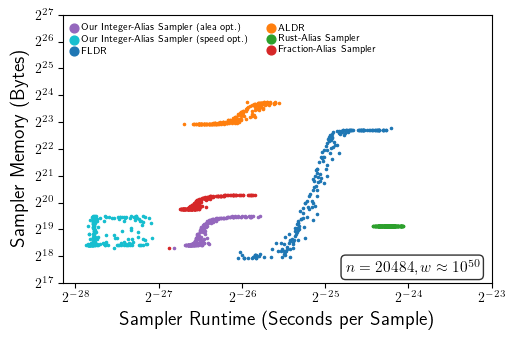
\includegraphics[width=0.48\textwidth]{figs/Runtime-memory.png}
    \hfill
    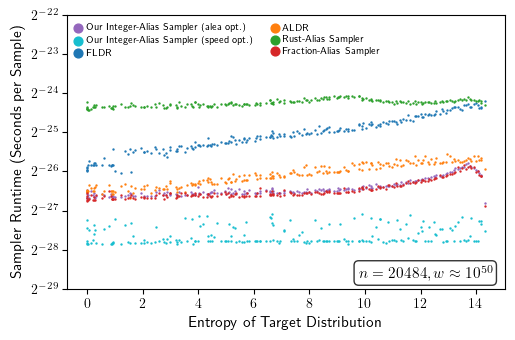
\includegraphics[width=0.48\textwidth]{figs/Entropy-runtime.png}
    \caption{Sampling runtime of the compared algorithms under arbitrary precision, against the memory footprint (left) and the entropy of the distributions (right)}
    \label{fig:runtime_memory}
\end{figure}

Figure~\ref{fig:runtime_memory} (left) plots the runtime of the sampling step against the memory footprint of the internal data structures, with each dot corresponding to one random distribution (averaged over 10 million samples). Remark that $2^{-20}\text{s} = 0.95\,\mu\text{s}$ and $2^{20}\text{B} = 1\text{MB}$. Beyond individual algorithm comparisons, the spread of each cluster is informative: the tight horizontal grouping of Alias-based methods reflects a fundamental algorithmic property, namely that their $O(1)$ sampling step is structurally independent of the target distribution, so every input distribution yields essentially the same runtime. By contrast, \textsc{Fldr} and \textsc{Aldr} exhibit a much wider horizontal spread, exposing their sensitivity to the shape of the distribution. The resulting picture traces an implicit Pareto frontier in the (runtime, memory) plane: \textsc{Fldr} and \textsc{Aldr} occupy the fast-but-memory-intensive region for favorable distributions, while Alias-based approaches occupy the compact-and-predictable region. Within the Alias family, our Integer-Alias Sampler consistently shifts the cluster to the left of Rust-Alias at comparable memory cost, demonstrating that integer normalization by $\mathtt{cs}$ rather than by the full cumulative weight $W$ produces a concrete speedup in the sampling step, independently of the distribution. Its v2 implementation is the fastest of all compared samplers, about $2.3$ times faster than v1 (median over the distributions).

Let us now make the entropy explicit as an independent variable to understand its role in the runtime, memory footprint, and preprocessing time.

\begin{figure}[ht]
    \centering
    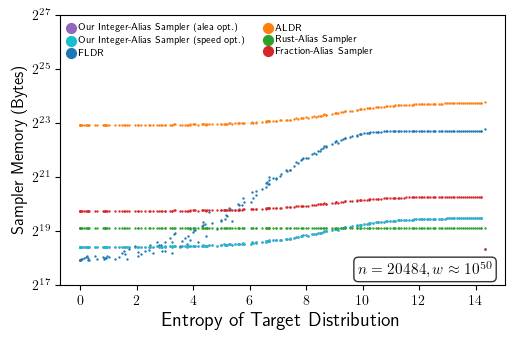
\includegraphics[width=0.48\textwidth]{figs/Entropy-memory.png}
    \hfill
    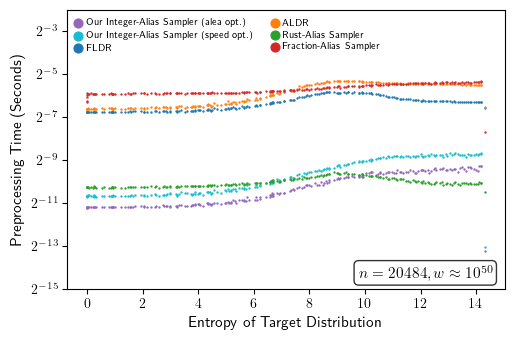
\includegraphics[width=0.48\textwidth]{figs/Entropy-preprocessing.png}
    \caption{Memory footprint (left) and preprocessing time (right) of the compared algorithms under arbitrary precision, as a function of the entropy of the distributions}
    \label{fig:memory_preprocessing}
\end{figure}

Figure~\ref{fig:runtime_memory} (right) confirms that Alias-based runtimes are near-constant across the full entropy spectrum. This invariance is not merely an empirical regularity: it is a direct consequence of the preprocessing step encoding the entire distribution into the alias table, so that each draw requires only a uniform bucket selection and a single Bernoulli test, regardless of the distributional complexity. The entropy-dependence of \textsc{Fldr} and \textsc{Aldr} has a different, more fundamental cause: both algorithms are built on the DDG-tree framework of Knuth and Yao~\cite{KY76}, in which random bits are consumed one at a time to navigate a binary decision tree. The expected number of bits per draw is approximately equal to the Shannon entropy of the distribution, and since each bit operation carries a fixed cost, the average runtime scales accordingly. As a result, \textsc{Fldr} and \textsc{Aldr} are \emph{faster} at low entropy (skewed distributions produce short, predictable tree paths) and \emph{slower} as entropy increases toward $\log_2(N)$ (near-uniform distributions require paths of maximal depth). The crossover at roughly half the maximum entropy (beyond which our Integer-Alias Sampler outperforms \textsc{Aldr} in runtime) reflects the point where the entropy-proportional cost of \textsc{Aldr} exceeds the constant cost of the Alias approach. The combinatorial chemistry application of Section~\ref{sec:chemie}, with its strongly skewed weight distribution falls in the low-entropy regime where \textsc{Fldr} and \textsc{Aldr} are at their most competitive; yet even there, our Integer-Alias Sampler remains within the same order of magnitude in runtime while providing strictly superior memory efficiency.

Regarding memory (Figure~\ref{fig:memory_preprocessing}, left), Alias-based approaches are more compact than \textsc{Aldr} across all entropies, and than \textsc{Fldr} except at low entropy, where its tree is small. Note that we report the exact memory footprint of the data structure produced by the preprocessing step. Within the Alias family, two observations are worth noting. First, even though the integer weights used by the Rust-Alias Sampler are $N$ times larger in value than those of our Integer-Alias Sampler (since Rust takes the total weight $W$ as the target cell capacity rather than $\mathtt{cs}$) the resulting table requires at most one additional cell, so both approaches yield similar memory footprints. Ours nevertheless grows with the entropy: our table stores each threshold with its significant bytes only, and the thresholds of light objects get longer as the distribution flattens. This confirms that the runtime advantage of Integer-Alias observed in Figure~\ref{fig:runtime_memory} (left) stems from the arithmetic cost of the Bernoulli step on large integers, not from a cache or layout effect. Second, the Fraction-Alias Sampler's table is approximately twice as large as those of the other Alias approaches: this is a direct consequence of storing exact rational numbers (numerator and denominator in arbitrary precision) rather than a single integer per entry, and it quantifies the memory cost of the more general rational representation.

Figure~\ref{fig:memory_preprocessing} (right) reports the preprocessing time, i.e., the construction of the data structure from the weights, file parsing excluded (for \textsc{Fldr}, whose construction is written in Python in~\cite{SFRM19}, we use a C port producing the same encoding). Our Integer-Alias Sampler, together with Rust-Alias, has the cheapest preprocessing: below $2.5$\,ms on every distribution, about twenty times less than \textsc{Fldr}, \textsc{Aldr} and the Fraction-Alias Sampler ($10$ to $25$\,ms). It only performs a linear number of integer operations on the weights, whereas \textsc{Fldr} and \textsc{Aldr} scan the binary expansion of every weight at each level of their DDG tree, and Fraction-Alias normalizes a rational number after each operation.

\begin{figure}[ht]
    \centering
    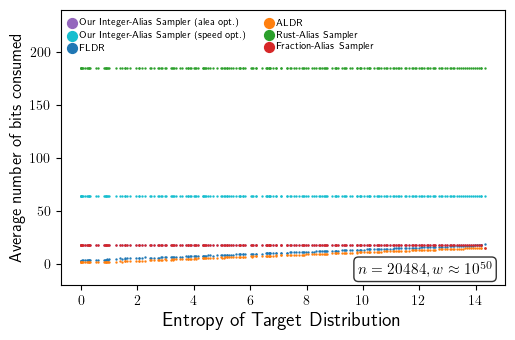
\includegraphics[width=0.48\textwidth]{figs/Entropy-bits.png}
    \hfill
    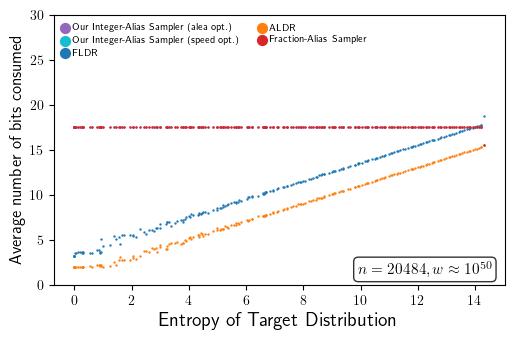
\includegraphics[width=0.48\textwidth]{figs/Entropy-bits2.png}
    \caption{Randomness consumption of the compared algorithms under arbitrary precision, as a function of the entropy of the distributions. The right plot zooms into the left one, capping the vertical axis at 30 bits}
    \label{fig:entropy_bits}
\end{figure}

Figure~\ref{fig:entropy_bits} reports the average number of random bits consumed per sample. The rightmost plot zooms into the leftmost one by capping the vertical axis at 30 bits, excluding Rust-Alias, whose consumption is an order of magnitude higher, and our v2 implementation ($64$ bits per draw). This anomaly has a structural cause: instead of sampling a Bernoulli variable, in the Rust approach requires drawing a uniform integer in $[0, W)$ where $\log_2(W) \approx 153$ bits (far beyond the $\log_2(N) \approx 14$ bits needed by our Integer-Alias Sampler). This is the direct price of the absence of weight normalization in the Rust implementation, and it renders that approach impractical for large-precision regimes regardless of its time efficiency.

Among the remaining four algorithms, \textsc{Fldr} and \textsc{Aldr} consume fewer random bits than our Integer-Alias Sampler across all entropies, with \textsc{Fldr} achieving the information-theoretic optimum of Knuth and Yao~\cite{KY76}. However, this entropic advantage narrows as entropy increases. In the high-entropy regime (distributions close to uniform), the dominant cost for any sampler is the uniform bucket selection, which requires $\log_2(N)$ bits regardless of the algorithm. As the distribution approaches uniform, this fixed cost dominates, and the overhead of our Integer-Alias Sampler relative to the optimum becomes negligible. In this limit, our algorithm thus simultaneously achieves $O(1)$ sampling time, minimal memory footprint, and near-optimal bit consumption (realizing, in the regime most favorable to all competing objectives, the best combination of all three efficiency criteria).



\begin{credits}
\subsubsection{\ackname} This work
	was supported by the \textsc{anr-fwf} project \textsc{PAnDAG} ANR-23-CE48-0014.

\subsubsection{\discintname}
The authors have no competing interests to declare that are relevant to the content of this article.
\end{credits}


%\newpage

%%
%% Bibliography
%%

{\raggedright % évite les blancs étirés devant les URL
\bibliography{parties/biblio}}
%%%%%%%%%%%%%%%%%%%%%%%%%%%%%%%%%%%%%%%%%%%%%%%%%%%%%%%%%%%%%%%%


%% On n'a pas le droit aux annexes 
% \newpage

% \appendix

% 
\section{Appendix dedicated to the optimal algorithms for $\textsc{Uniform}$ and $\textsc{Bernoulli}$ functions}
\label{app:lumbroso}

\noteAnt{mettre un peu de blabla}

\begin{algorithm}[htb]
\caption{Generating a random integer} 
\label{algo:tableXX}
	\begin{algorithmic}[1]
        \renewcommand{\algorithmicrequire}{\textbf{Input:}}
        \renewcommand{\algorithmicensure}{\textbf{Output:}}
        \Require $n$, the upper limit (excluded)
        \Ensure  A random number between $0$ and $n-1$.
        \Function{rand\_int}{$n$}
            \While{True}
                \State $res = 0$
                \State $bits = n.bit\_length()$ \Comment{Return the number of necessary bits to represent the integer in binary}
                \For{$i=0 \text{ to } bits$}
                    \State $res = res * 2 + randint(0, 1)$ \Comment{Add the bit generated}
                \EndFor
                \If{$res < n$}
                    \State \Return $res$
                \EndIf
            \EndWhile
        \EndFunction
	\end{algorithmic}   
 \end{algorithm}

\begin{algorithm}[htb]
\caption{Random sampling in $\bar{T}$} 
\label{algo:tableXY}
	\begin{algorithmic}[1]
        \renewcommand{\algorithmicrequire}{\textbf{Input:}}
        \renewcommand{\algorithmicensure}{\textbf{Output:}}
        \Require $\bar{T}$, $\cs, \bar{q}$  previously defined.
        \Ensure A random object from $\bar{T}$
        \Function{RandomGeneration}{$\bar{T}$, $\cs, \bar{q}$}
            \State $q1 = \bar{q} - 1$
            \State $q2 = \bar{q} - 2$
            \While{True}
                \State $r = \texttt{rand\_int}(\bar{q})$
                \State $box = \bar{T}[r]$
                \If{$0 \leq r \leq q2$} \Comment{First part of the table $\bar{T}$}
                    \State $r' = \texttt{rand\_int}(cs)$
                    \If{$r' \leq box[0]$}
                        \State \Return $box[1]$
                    \Else
                        \State \Return $box[2]$
                    \EndIf
                \ElsIf{$r == q1$} \Comment{Last box of the table $\bar{T}$ : there is potentially a virtual object}
                    \State $r' = \texttt{rand\_int}(cs)$
                    \If{$r' \leq box[0]$}
                        \State \Return $box[1]$
                    \EndIf
                \EndIf
            \EndWhile
        \EndFunction
    \end{algorithmic}
\end{algorithm}




\section{Appendix dedicated to the Combinatorial Chemistry case study}
\label{app:chemistry}
\noteAnt{A nettoyer, des choses ont déjà été dites dans corps du papier}

\paragraph{Introduction and Problem Statement}
Weighted random sampling is a fundamental operation in scientific computing. It consists in selecting an item $x_i$ from a set of $n$ candidates $X = \{x_0, x_1, \dots, x_{n-1}\}$ with probability strictly proportional to its integer weight $w_i$:
\begin{equation}
\mathbb{P}(X = x_i) = \frac{w_i}{\text{total}}
\end{equation}

\noteAnt{il y a qq chose de commenter qui ne compile pas, mais est iportant à mettre en place}
% counter = ncs.ApproximateCounter(show_progress=False)\\
% space = ncs.SearchSpace("C:4 H:1 O:2 N:3 F:1") ## ce sont les valences correctes présentes dans la nature -- vallence == nb de liaisons // dans l'exemple précédent on autorisait des valences + importantes\\
% mols = ncs.random_sample(
%     counter, space, natoms=32, nmols=1, selection=ncs.Q("C + H + O + N + F = 32")
% )}
% $N = 20\,484$; $Z = 467734548828719531605240429605504136894484614517198 \sim 1.25 \cdot 2^{168} \sim 4.7 \cdot 10^{50}$.


\paragraph{Floating-Point Arithmetic Bias: Why \texttt{random.uniform} is Not Uniform}
In Python, the standard implementation for cumulative weighted sampling draws a continuous random variable $r \sim \mathcal{U}[0, \text{total})$ and searches for the corresponding cumulative range. Within Python's standard library (\texttt{random.choices}), sampling relies on calling \texttt{random.uniform(0, total)} or \texttt{random() * total}. The weighted sampling step (5) is implemented in \texttt{nablachem/space/algos.py} as shown in Figure~4:

% [FIGURE 4: Chemistry sampling code snippet (_weighted_choose)]

Although \texttt{total} is accumulated using Python's arbitrary-precision integers (\texttt{int}), evaluating \texttt{random.uniform(0, total)} implicitly converts this integer mass into an IEEE 754 double-precision float (\texttt{float64}). An IEEE 754 \texttt{float64} value allocates 52 explicit mantissa bits plus 1 implicit bit, granting $M = 2^{53}$ distinct representable values in $[0, 1)$.

As long as $\text{total} \le 2^{53}$, every integer index possesses an exact floating-point representation. However, as soon as $\text{total} > 2^{53}$, the step size between consecutive representable floating-point values becomes strictly greater than $1$:
\begin{itemize}
    \item Between $2^{53}$ and $2^{54}$, the step size is $2^1 = 2$: only even integers can be reached.
    \item Between $2^{54}$ and $2^{55}$, the step size is $2^2 = 4$: only multiples of 4 are reachable.
    \item For $\text{total} \sim 2^{100}$, the step size between consecutive draws leaps to $2^{47} \approx 1.4 \times 10^{14}$.
\end{itemize}

Let $M = 2^{\text{bits}}$ be the number of representable values for a uniform floating-point number $f \in [0, 1)$, and $\text{total}$ be the total weight of the distribution:
\begin{itemize}
    \item \textbf{Regime $M \gg \text{total}$ (sufficient precision):} Discretization error is limited to minor rounding noise.
    \item \textbf{Regime $M \ll \text{total}$ (large-scale real-world case, e.g., $M = 2^{53}, \text{total} \sim 2^{100}$):} The resolution step $\text{total}/M$ exceeds the individual weights of many candidate items. An item whose weight is smaller than this grid resolution incurs a selection probability that becomes \emph{structurally zero}, regardless of its non-zero theoretical probability.
\end{itemize}

To quantify this deviation exactly without resorting to expensive Monte Carlo simulations, an $O(n)$ exact arithmetic algorithm calculates the effective probability distribution reachable for a target bit precision. By evaluating how many grid points $f = k/M$ (projected as $f \times \text{total}$) land within each item's cumulative interval, the algorithm computes effective sampling weights using integer division with ceiling, completely independent of the magnitude of $\text{total}$.

% [FIGURE 5: Stretching and shrinking of a finite-precision random source (M=16)]

Figure~5 illustrates these discretization mechanics using 4-bit precision ($M = 16$, center axis):
\begin{itemize}
    \item \textbf{Stretched regime ($M < \text{total}$, top axis, blue):} The 16 available values are stretched over 22 target integer slots. Because the resolution step ($22/16 = 1.375$) is strictly greater than 1, covering every target integer is impossible. Gaps remain: items falling entirely into these gaps have a zero probability of being chosen.
    \item \textbf{Shrunk regime ($M > \text{total}$, bottom axis, orange):} The 16 values are compressed over 10 target integer slots. The average step ($16/10 = 1.6$) allows every target to be reached. However, since 10 does not divide 16, grid points stack unevenly, assigning two points to certain targets and one to others, inducing a modulo bias.
\end{itemize}

\paragraph{Advantages of the Integer ALIAS Method in Arbitrary Precision}
The ALIAS method using arbitrary-precision integers provides an optimal solution to address both precision errors during sampling and execution time bottlenecks.

First, this method guarantees complete mathematical exactness. By operating exclusively with arbitrary-precision integers, it preserves the exact weight of every item regardless of scale. The resulting draws remain strictly unbiased and faithful to the theoretical distribution.

Second, it provides significant speedups. Linear scanning methods iterate through weights sequentially, incurring an $O(n)$ sampling time per draw. Across millions of trials, this becomes prohibitive. Our ALIAS approach resolves this by building a lookup table once during a preprocessing step, after which every subsequent draw executes in $O(1)$ constant time.

In summary, arbitrary-precision integer ALIAS eliminates floating-point conversion errors while enabling instant random sampling, making it ideal for massive combinatorial spaces.




\section{Lumbroso's sampling algorithms}


\noteAnt{Algo de Lumbroso \cite{Lumbroso13}}
\begin{algorithm}[H]
\caption{Generating a random integer or a Bernoulli variable} 
\label{algo:RandInt_v_AI}
    \begin{tabular}{l l}
        \begin{minipage}{0.5\textwidth}
	        \begin{algorithmic}[1]
                \renewcommand{\algorithmicrequire}{\textbf{Input:}}
                \renewcommand{\algorithmicensure}{\textbf{Output:}}
                \Require $n$, the upper limit (excluded)
                \Ensure  A uniform random integer between $0$ and $n-1$.
                \Function{\textsc{Uniform}}{$n$}
                    \State $k = \lceil \log_2(n) \rceil$
                    \State $bound = 2^k$
                    \State $x = \texttt{Rand\_Bits}(k)$
                    \While{$bound < n$ \textbf{or} $x \geq n$}
                        \If{$bound \geq n$}
                            \State $bound = bound - n$
                            \State $x = x - n$
                        \EndIf
                        \State $bound = 2 \cdot bound$
                        \State $x = 2 \cdot x + \texttt{Rand\_Bits}(1)$
                    \EndWhile
                    \State \Return $x$
                \EndFunction
	        \end{algorithmic}
        \end{minipage}
        &
        \begin{minipage}{0.5\textwidth}
            \begin{algorithmic}[1]
                \renewcommand{\algorithmicrequire}{\textbf{Input:}}
                \renewcommand{\algorithmicensure}{\textbf{Output:}}
                \Require $p, q$ with $0 \leq p \leq q$
                \Ensure  A Bernoulli variable equal to $1$ with probability $p/q$.
                \Function{\textsc{Bernoulli}}{$p, q$}
                    \If{$p = q$}
                        \State \Return $1$
                    \EndIf
                    \State $p = 2 \cdot p$
                    \While{$p \neq q$}
                        \If{$p > q$}
                            \State $y = 1$
                            \State $p = p - q$
                        \Else
                            \State $y = 0$
                        \EndIf
                        \If{\texttt{Rand\_Bits}(1) == 1}
                            \State \Return $y$
                        \EndIf
                        \State $p = 2 \cdot p$
                    \EndWhile
                    \State \Return \texttt{Rand\_Bits}(1)
                \EndFunction
            \end{algorithmic}
        \end{minipage}
    \end{tabular}
    \begin{itemize}
        \footnotesize 
        \item $\texttt{Rand\_Bits}(k)$: it returns an integer whose base-2 representation is built with a sequence of $k$ unbiased random bits
    \end{itemize}
 \end{algorithm}



\end{document}
